\documentclass[12pt,letterpaper]{article}

% \input{worksheet-setup.tex}
\usepackage{fancyhdr,fancybox}
\usepackage{amsmath}
\usepackage{amsthm}
\usepackage{amssymb}
\usepackage{tikz}

\usepackage{enumitem}
\usepackage{multicol}
\usepackage[export]{adjustbox}

%% Useful packages
\usepackage{amssymb, amsmath, amsthm} 
%\usepackage{graphicx}  %%this is currently enabled in the default document, so it is commented out here. 
\usepackage{calrsfs}
\usepackage{braket}
\usepackage{mathtools}
\usepackage{lipsum}
\usepackage{tikz}
\usetikzlibrary{cd}
\usepackage{verbatim}
%\usepackage{ntheorem}% for theorem-like environments
\usepackage{mdframed}%can make highlighted boxes of text
%Use case: https://tex.stackexchange.com/questions/46828/how-to-highlight-important-parts-with-a-gray-background
\usepackage{wrapfig}
\usepackage{centernot}
\usepackage{subcaption}%\begin{subfigure}{0.5\textwidth}
\usepackage{pgfplots}
\pgfplotsset{compat=1.13}
\usepackage[colorinlistoftodos]{todonotes}
\usepackage[colorlinks=true, allcolors=blue]{hyperref}
\usepackage{xfrac}					%to make slanted fractions \sfrac{numerator}{denominator}
\usepackage{enumitem}            
    %syntax: \begin{enumerate}[label=(\alph*)]
    %possible arguments: f \alph*, \Alph*, \arabic*, \roman* and \Roman*
\usetikzlibrary{arrows,shapes.geometric,fit}

\DeclareMathAlphabet{\pazocal}{OMS}{zplm}{m}{n}
%% Use \pazocal{letter} to typeset a letter in the other kind 
%%  of math calligraphic font. 

%% This puts the QED block at the end of each proof, the way I like it. 
\renewenvironment{proof}{{\bfseries Proof}}{\qed}
\makeatletter
\renewenvironment{proof}[1][\bfseries \proofname]{\par
  \pushQED{\qed}%
  \normalfont \topsep6\p@\@plus6\p@\relax
  \trivlist
  %\itemindent\normalparindent
  \item[\hskip\labelsep
        \scshape
    #1\@addpunct{}]\ignorespaces
}{%
  \popQED\endtrivlist\@endpefalse
}
\makeatother

%% This adds a \rewnewtheorem command, which enables me to override the settings for theorems contained in this document.
\makeatletter
\def\renewtheorem#1{%
  \expandafter\let\csname#1\endcsname\relax
  \expandafter\let\csname c@#1\endcsname\relax
  \gdef\renewtheorem@envname{#1}
  \renewtheorem@secpar
}
\def\renewtheorem@secpar{\@ifnextchar[{\renewtheorem@numberedlike}{\renewtheorem@nonumberedlike}}
\def\renewtheorem@numberedlike[#1]#2{\newtheorem{\renewtheorem@envname}[#1]{#2}}
\def\renewtheorem@nonumberedlike#1{  
\def\renewtheorem@caption{#1}
\edef\renewtheorem@nowithin{\noexpand\newtheorem{\renewtheorem@envname}{\renewtheorem@caption}}
\renewtheorem@thirdpar
}
\def\renewtheorem@thirdpar{\@ifnextchar[{\renewtheorem@within}{\renewtheorem@nowithin}}
\def\renewtheorem@within[#1]{\renewtheorem@nowithin[#1]}
\makeatother

%% This makes theorems and definitions with names show up in bold, the way I like it. 
\makeatletter
\def\th@plain{%
  \thm@notefont{}% same as heading font
  \itshape % body font
}
\def\th@definition{%
  \thm@notefont{}% same as heading font
  \normalfont % body font
}
\makeatother

%===============================================
%==============Shortcut Commands================
%===============================================
\newcommand{\ds}{\displaystyle}
\newcommand{\B}{\mathcal{B}}
\newcommand{\C}{\mathbb{C}}
\newcommand{\F}{\mathbb{F}}
\newcommand{\N}{\mathbb{N}}
\newcommand{\R}{\mathbb{R}}
\newcommand{\Q}{\mathbb{Q}}
\newcommand{\T}{\mathcal{T}}
\newcommand{\Z}{\mathbb{Z}}
\renewcommand\qedsymbol{$\blacksquare$}
\newcommand{\qedwhite}{\hfill\ensuremath{\square}}
\newcommand*\conj[1]{\overline{#1}}
\newcommand*\closure[1]{\overline{#1}}
\newcommand*\mean[1]{\overline{#1}}
%\newcommand{\inner}[1]{\left< #1 \right>}
\newcommand{\inner}[2]{\left< #1, #2 \right>}
\newcommand{\powerset}[1]{\pazocal{P}(#1)}
%% Use \pazocal{letter} to typeset a letter in the other kind 
%%  of math calligraphic font. 
\newcommand{\cardinality}[1]{\left| #1 \right|}
\newcommand{\domain}[1]{\mathcal{D}(#1)}
\newcommand{\image}{\text{Im}}
\newcommand{\inv}[1]{#1^{-1}}
\newcommand{\preimage}[2]{#1^{-1}\left(#2\right)}
\newcommand{\script}[1]{\mathcal{#1}}


\newenvironment{highlight}{\begin{mdframed}[backgroundcolor=gray!20]}{\end{mdframed}}

\DeclarePairedDelimiter\ceil{\lceil}{\rceil}
\DeclarePairedDelimiter\floor{\lfloor}{\rfloor}

%===============================================
%===============My Tikz Commands================
%===============================================
\newcommand{\drawsquiggle}[1]{\draw[shift={(#1,0)}] (.005,.05) -- (-.005,.02) -- (.005,-.02) -- (-.005,-.05);}
\newcommand{\drawpoint}[2]{\draw[*-*] (#1,0.01) node[below, shift={(0,-.2)}] {#2};}
\newcommand{\drawopoint}[2]{\draw[o-o] (#1,0.01) node[below, shift={(0,-.2)}] {#2};}
\newcommand{\drawlpoint}[2]{\draw (#1,0.02) -- (#1,-0.02) node[below] {#2};}
\newcommand{\drawlbrack}[2]{\draw (#1+.01,0.02) --(#1,0.02) -- (#1,-0.02) -- (#1+.01,-0.02) node[below, shift={(-.01,0)}] {#2};}
\newcommand{\drawrbrack}[2]{\draw (#1-.01,0.02) --(#1,0.02) -- (#1,-0.02) -- (#1-.01,-0.02) node[below, shift={(+.01,0)}] {#2};}

%***********************************************
%**************Start of Document****************
%***********************************************
 %find me at /home/trevor/texmf/tex/latex/tskpreamble_nothms.tex

%%
%% Page set-up:
%%
\pagestyle{empty}
\lhead{\textsc{34A - Units, Areas, Volumes, Lines}} %=================UPDATE THIS=================%
\rhead{\textsc{Winter 2020}}
%\chead{\Large\textbf{A New Integration Technique \\ }}
\rfoot{trevorklar@math.ucsb.edu}
\renewcommand{\headrulewidth}{1pt}

\setlength{\parindent}{0in}
\setlength{\textwidth}{7in}
\setlength{\evensidemargin}{-0.25in}
\setlength{\oddsidemargin}{-0.25in}
\setlength{\parskip}{.5\baselineskip}
\setlength{\topmargin}{-0.5in}
\setlength{\textheight}{9in}

\setlist[enumerate,1]{label=\textbf{\arabic*.}}

\begin{document}
\thispagestyle{fancy}
\begin{center}
3B - Calculus for Social and Life Sciences\\
Week 2 %=================UPDATE THIS=================%
\end{center}

\hrule

\begin{center}
\begin{tabular}{|rl|}
\hline
\multicolumn{2}{|c|}{Contact Information} \\
\hline
\bf{TA's name:} & Trevor Klar \\
\bf{Email:} & trevorklar@math.ucsb.edu \\
\bf{Office hours:} & Wednesdays 2:00-3:00 \\
\bf{Math Lab hours:} & Tuesdays 3:00-5:00 \\
\bf{Office:} & South Hall 6431x \\
\hline
\end{tabular}
\end{center}

 %=================START OF WORKSHEET=================%

%Helpful hi9nts and formulas go here
\bigskip

\begin{enumerate}

\item \mbox{} I was born on the second day\\
\hspace*{.5em} of the last week\\
\hspace*{1em} of the second to last month\\
\hspace*{1.5em}   of the last year\\
\hspace*{2em}    of the second to last decade\\
\hspace*{2.5em}     of the last century\\
\hspace*{3em}      of the second millennium\\
\hspace*{3.5em}       of our calendar system. 

 \mbox{} What is my birthdate?
\vfill

%\end{enumerate}

%\begin{minipage}{.7\linewidth}
%\begin{enumerate} \setcounter{enumi}{3}
\item A goblin catapult sits at at the top of a 200 foot cliff, overlooking the enemy. When it launches, the height of its "projectile" (see figure) is given by the equation $f(t)=-16t^2+200$, where $t$ is the time in seconds since launch and $f(t)$ is the height of the projectile above the enemy. How long will we be able to hear the projectile cackling maniacally until it strikes the target? [Hint: We want to know what value of $t$ makes $f(t)=0$, so find the inverse of the function.]
%\end{enumerate}
%\end{minipage} 
%\begin{minipage}{.3\linewidth}
%\jpg{width=.3\linewidth}{goblin_cannon}
%\begin{figure}[h]
\vspace*{-3ex}
\hfill
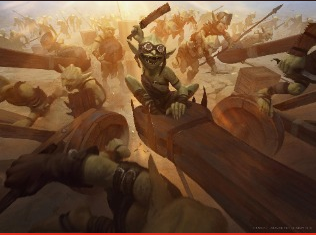
\includegraphics[width=.3\linewidth,right]{goblin_cannon}
%\caption{Goblin catapult}
%\end{figure}
%\end{minipage}
\vspace*{-1.5in}
\vfill

\pagebreak
\item A really rich guy wants to decorate his garage door with 14K gold Christmas tree lights, illuminating the top and sides of his door. His door has an area of 112 square feet, and the lights cost \$295 per meter. Express the total cost of the Christmas lights in terms of the width of the garage door. (There are about 3.28 feet in 1 meter). 
\vfill

\item Solve $\dfrac{x^2-3}{x+2}-x=4$. \quad [Hint: First get a common denominator.]
\vfill 

%\begin{enumerate} \setcounter{enumi}{4}
\item I have three numbers. The middle one is half the biggest one,
and the smallest one plus the middle one is four less than
the biggest one. The biggest one plus the middle one is five times the smallest one.  What are the numbers?
\vfill




\end{enumerate}




\end{document}


%%% Local Variables: 
%%% mode: latex
%%% TeX-master: t
%%% End: 
